\documentclass[11pt,a4paper,oneside]{book}
\newcommand{\NumeroRelazione}{2}

\newcommand{\TitoloRelazione}{Misure con l'analizzatore di spettro}
\usepackage[utf8]{inputenc}       
\usepackage[T1]{fontenc}          
\usepackage[italian]{babel}       
\usepackage{graphicx}             
\usepackage{float}
\usepackage{amsmath}
\usepackage{amsfonts} 
\usepackage{amssymb}  
\usepackage{steinmetz}
\usepackage{pgfplots}
\usepackage{tikz}
\usepackage{enumitem} 
\usepackage{subcaption}
\usepackage{caption}
\usepackage[normalem]{ulem}
\usepackage[americaninductors, siunitx]{circuitikz}

\usetikzlibrary{arrows.meta, patterns, shapes.geometric, calc, positioning, shapes, arrows}
\pgfplotsset{compat=1.18}

% --- GEOMETRY (Margini e distanze) ---
\usepackage[
    a4paper,
    top=3.5cm,      
    bottom=3cm,    
    left=3cm,      
    right=3cm,     
    headheight=40pt, % Spazio per l'immagine
    headsep=25pt     % Distanza tra immagine e testo/titoli
]{geometry}

% --- FANCYHDR (Intestazioni) ---
\usepackage{fancyhdr} 
\pagestyle{fancy}
\fancyhf{} 
\fancyhead[L]{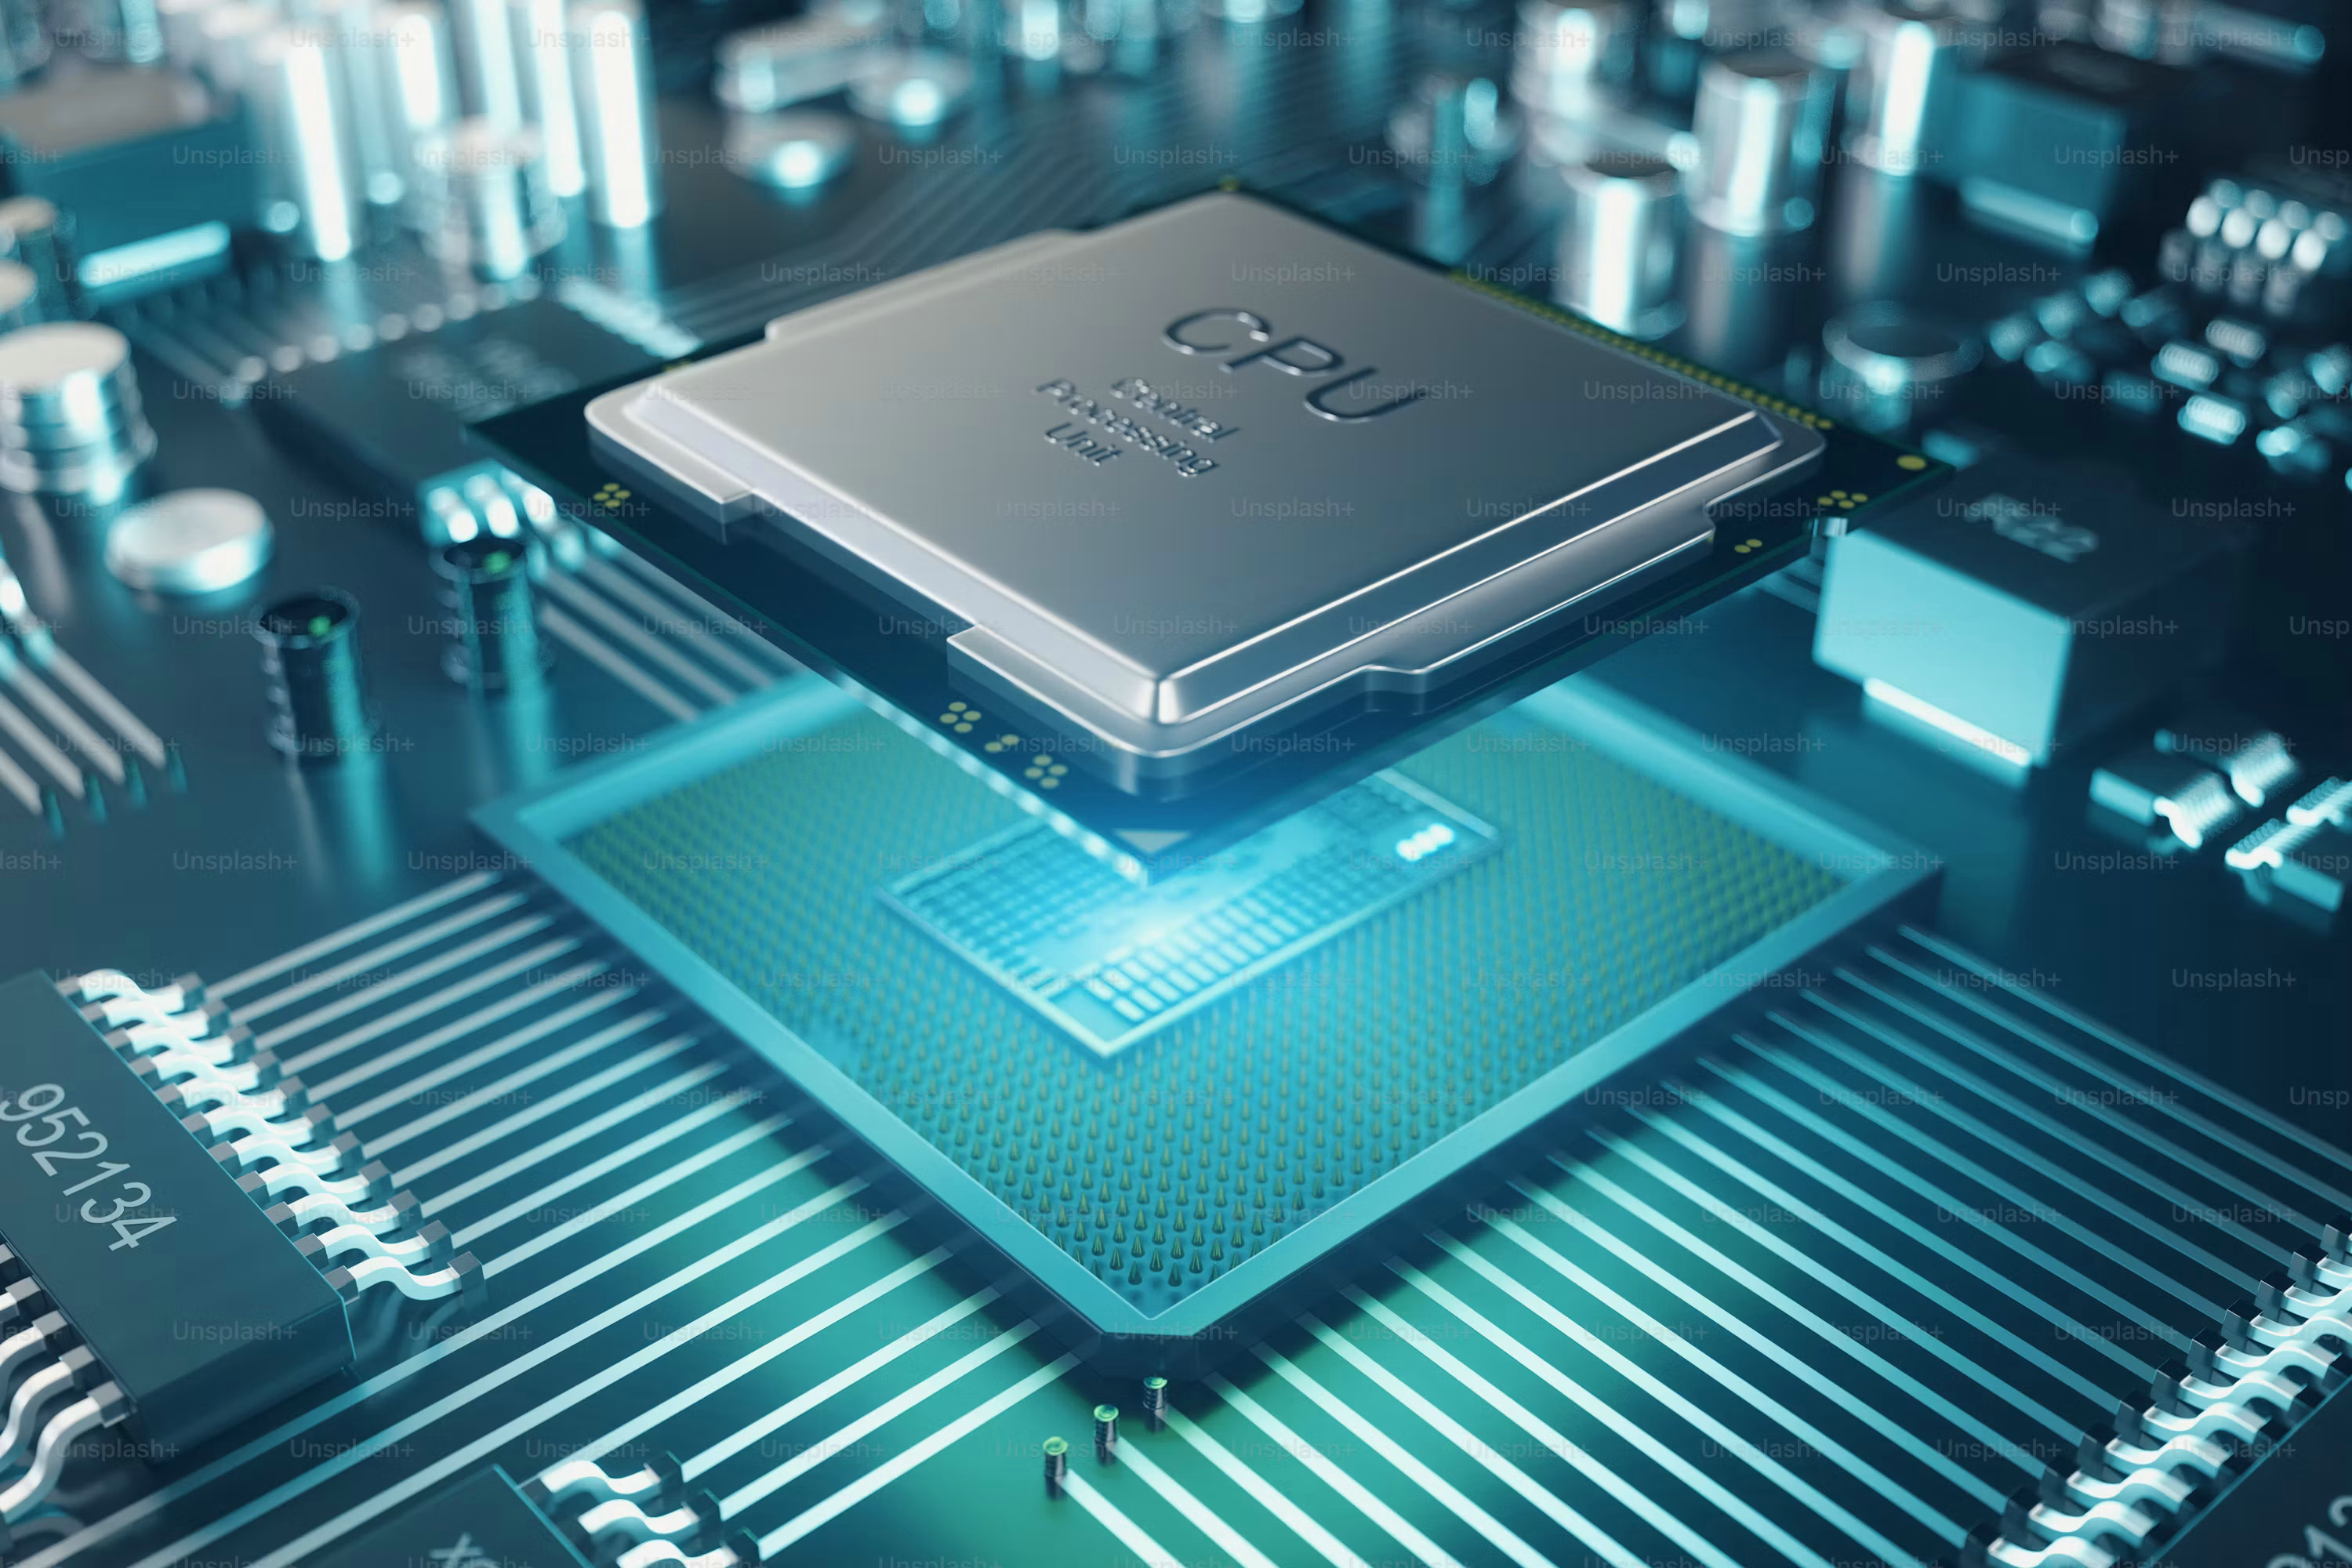
\includegraphics[height=1cm]{Images/top.png}} 
\fancyhead[R]{\thepage} 
\fancyhead[C]{\textit{\leftmark}} 

% Per avere l'intestazione anche nelle pagine iniziali dei capitoli
\fancypagestyle{plain}{
  \fancyhf{}
  \fancyhead[L]{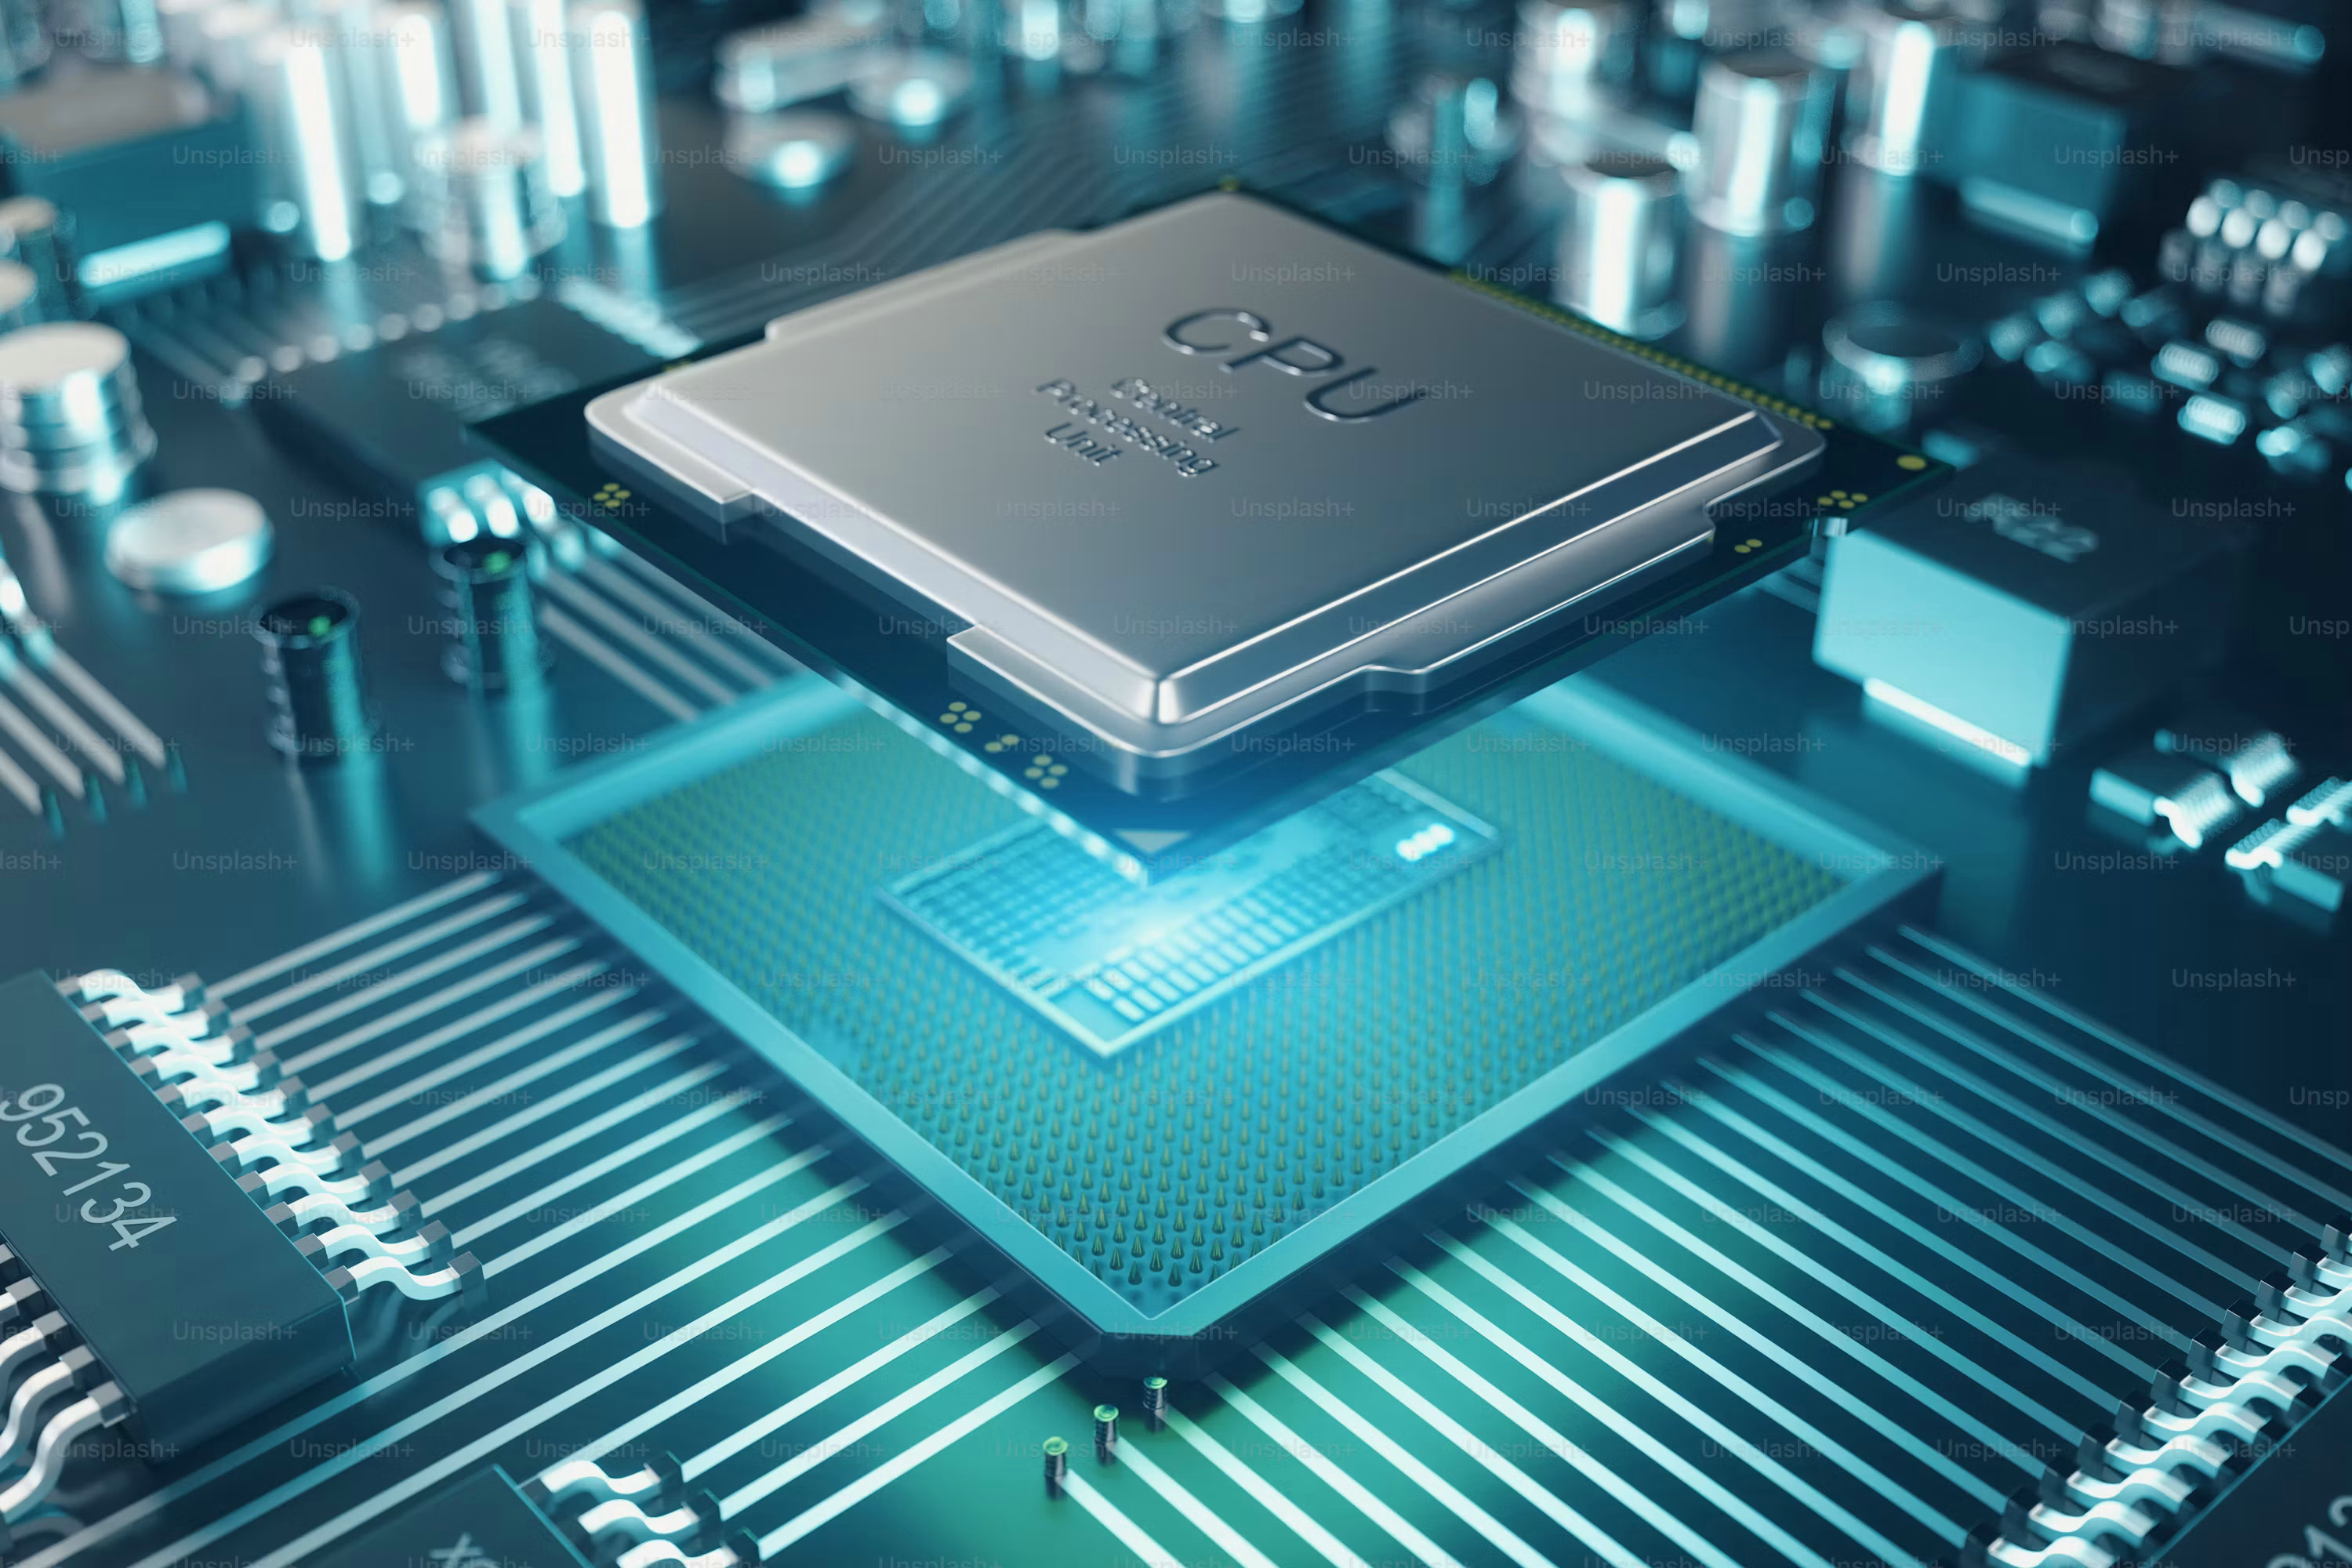
\includegraphics[height=1cm]{Images/top.png}}
  \fancyhead[R]{\thepage}
  \fancyhead[C]{\textit{\leftmark}}
  \renewcommand{\headrulewidth}{0.4pt}
}

% --- LINK CLICCABILI (Senza il backtick d'errore) ---
\usepackage[hidelinks]{hyperref} 
 

% --- COMANDI PERSONALIZZATI ---
\newcommand{\tikznode}[2]{%
  \ifmmode%
    \tikz[remember picture,baseline=(#1.base),inner sep=0pt] \node (#1) {$#2$};%
  \else
    \tikz[remember picture,baseline=(#1.base),inner sep=0pt] \node (#1) {#2};%
  \fi%
}
\tikzset{portnode/.style={circle, draw, inner sep=1pt, font=\scriptsize}}


\begin{document}
% --- PAGINA DEL TITOLO 
\begin{titlepage}
    \centering
    {\scshape\Large Università degli Studi "La Sapienza" \par} 
    \vspace{0.5cm}
    {\scshape\large Dipartimento di Ingegneria dell'Informazione, Elettronica e Telecomunicazioni \par}
    \vspace{0.5cm}
    {\scshape\large Corso di Laurea in Ingegneria Elettronica \par}
    \vspace{1.5cm}
    {\huge\bfseries Laboratorio Multidisciplinare\\ di Elettronica I\par}
    \vspace{0.35cm}
    {\Large\bfseries Relazione \NumeroRelazione\par}
    \vspace{0.35cm}
    {\Large\bfseries \TitoloRelazione\par}
    \vspace{1cm}
    {\large CFU:  6 \par} 
    \vspace{1.5cm}

    {\large Gruppo 18: \par}
    \vspace{0.2cm}
    {\Large Renato Bearzotti \par}
    {\Large Nicolò Falasca \par}
    {\Large Ionut Vlase }

    \vspace{0.6cm}
    \IfFileExists{Images/top.png}{%
        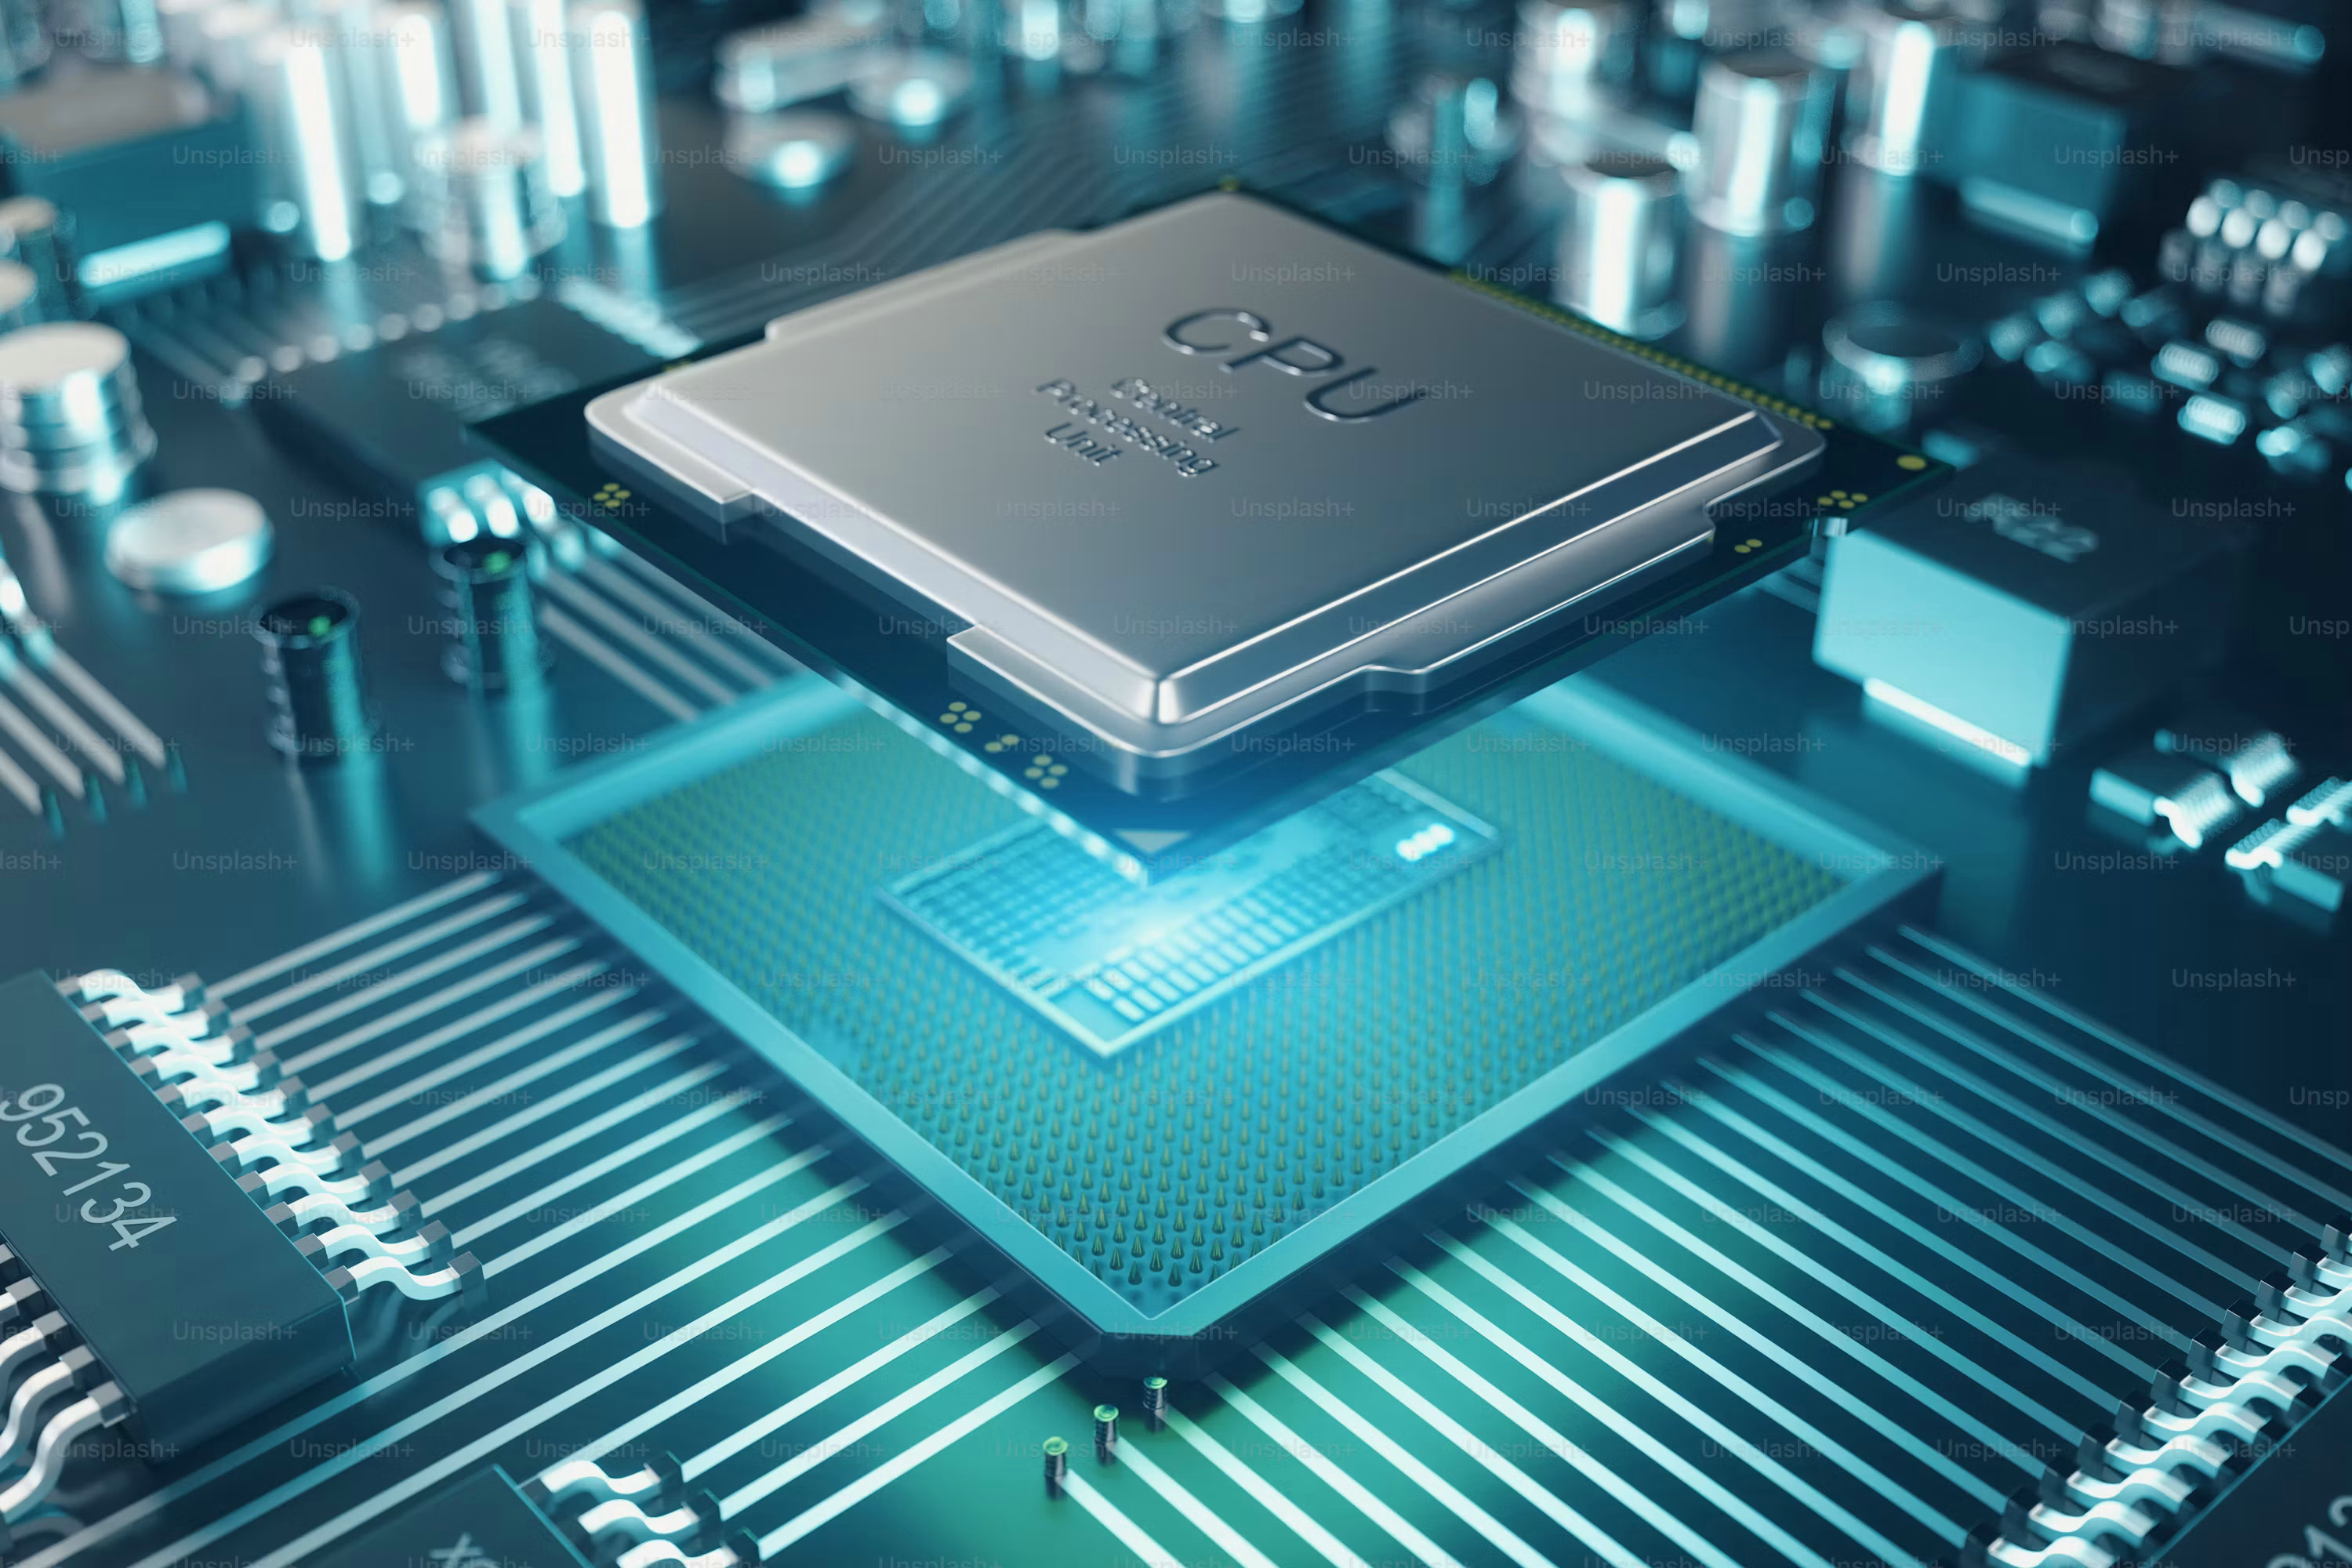
\includegraphics[width=3.5cm]{Images/top.png}\par
    }{}
    \vspace{0.35cm}
    \IfFileExists{Images/logo Sapienza (rgb).png}{%
        
\includegraphics[width=6.8cm]{Images/logo Sapienza (rgb).png}\par
    }{}
    \vspace{0.8cm}

    % Professori allineati a destra
    \begin{minipage}[t]{\textwidth}
        \begin{flushright}
            \large
            \textbf{Professori:}\\
            Andrea Mostacci\\
            Stefano Pisa\\
            Pasquale Tommasino
        \end{flushright}
    \end{minipage}

    \vfill
    {\large Anno Accademico 2026-2027 \par}
\end{titlepage}


\frontmatter 
\tableofcontents

\mainmatter
 \chapter{Note!!! do,re,mi,fa,sol,la ,si do}
Rifai figura 3.1, sinusuoide, con marker, e riedi conti. 
\\incertezza SPA?? Rivedi cifre dopo la virgola
\chapter{Misura della frequenza e dell'ampiezza di un segnale sinusoidale con incertezza}

\chapter{Misura del DANL}

\chapter{Spettro di segnali elementari}
Per questa valutazione di laboratorio abbiamo usato il generatore di segnali per generare vari 
segnali periodici a 1MHz di frequenza e con ampiezza di picco di 1V (2V di ampiezza picco-picco).
\\In ogni misurazione con lo SPA abbiamo prima verificato il segnale del generatore tramite
 l'oscilloscopio digitale, in modo da avere una verifica preliminare del segnale generato
 tramite uno strumento a noi più consono. 
\\Per tutte le misurazioni il generatore di segnale è stato impostato come impedenza di
 uscita $50\Omega$, poichè con il generatore usato si può impostare l'impedenza di uscita a
 $50\Omega$ oppure a "High Impedence". Ovviamente la scelta è stata fatta poiché il nostro SPA ha
una impedenza di ingresso di $50\Omega$, e in questo modo abbiamo ottenuto il massimo
 adattamento, e coefficiente di riflessione nullo.

\section{Misurazione di un segnale sinusoidale con oscilloscopio e SPA}
In questo caso abbiamo usato il generatore per ottenere un segnale sinusoidale con le specifiche 
viste sopra. Per queste misurazioni abbiamo impostato la RBW a 1KHz, minimizzando anche qui il
 rumore senza ottenere variazioni del segnale o misurazioni troppo lente) e lo span a 50KHz.
\\Per la misurazione abbiamo impostato il generatore a 1V di tensione picco-picco, poichè in questo
 caso il generatore, senza carico interno, generain maniera autonoma  una sinusoide a 2V di picco-picco,
 in modo che una volta attaccato a un carico da $50 \Omega$, come nel caso del SPA, sullo strumento
 arrivi metà della tensione del generatore in aperto. La Figura~\ref{fig:circuito_50ohm} mostra il
 circuito equivalente appena esposto.
\\ Quindi, per vedere sull'oscilloscopio, che ha
 una impedenza di ingresso elevata ($1M\Omega$), un segnale a 1V di picco come da specifica
dell'esercitazione abbiamo impostato il generatore a 1V di tensione picco-picco.

\begin{figure}[H]
    \centering
    \begin{circuitikz}[american voltages]
        \draw
        (0,0) to[V, invert, l=$V_1$] (0,3)
              to[R, l={$R_1=50\,\Omega$}] (3,3)
              to[short, -*] (4,3)
              to[R, l={$R_L=50\,\Omega$}] (4,0)
              -- (0,0);

        % Nodo dopo la prima resistenza
        \node[above] at (4,3) {$V_L$};

        % Riferimento di massa
        \draw (2,0) node[ground]{};
    \end{circuitikz}

    \caption{Circuito con generatore e carico da 50 ohm.}
    \label{fig:circuito_50ohm}
\end{figure}

Siamo passati poi a misurare il segnale con lo SPA e il segnale ottenuto è il seguente. Come nel
caso precedente, per ottenere il segnale desiderato, abbiamo valutato la tensione picco-picco del
generatore da inserire in base all'impedenza di ingresso dello strumento di misura. Abbiamo quindi 
impostato la tensione picco-picco del generatore a 1V, in modo da avere una sinusoide a 1V picco-picco
in ingresso allo SPA. 
\\La misura è riportata nella Figura~\ref{fig:sinusoide_1MHz}.

\begin{figure} [H]
\centering
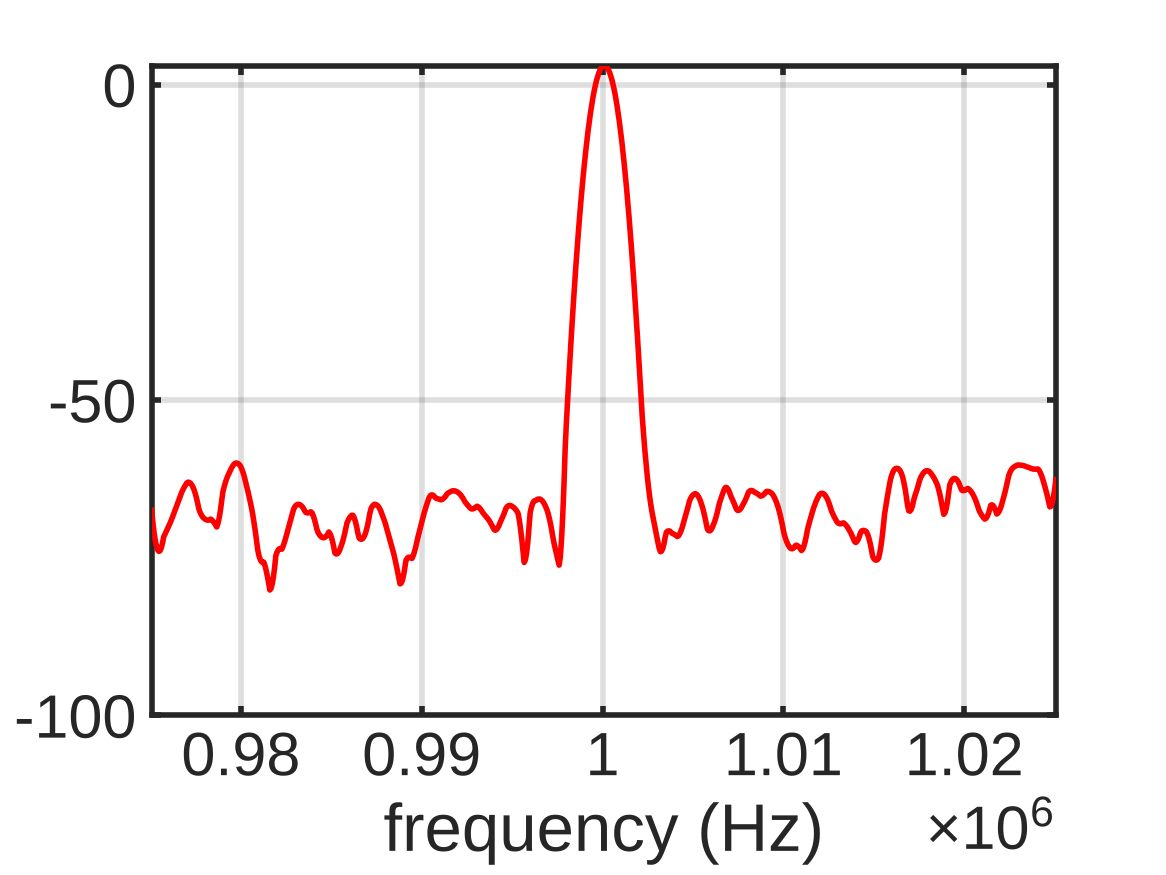
\includegraphics[width=0.6\textwidth]{./Images/Relazione2_Foto/3_1_sinusioide_1MHz_Vp=1_span_50KHz.jpeg}
\caption{Segnale sinuoidale misurato tramite lo SPA.}
\label{fig:sinusoide_1MHz}
\end{figure}
Il valore misurato  a $1.0000\pm 0.0012 MHz$ è $3.01dBm\pm+0.5 dB$.
\\Prima di misurare ci aspettavamo dalla teoria un valore di circa 3.98dBm. Questo valore è stato
 ricavato tramite i seguenti passaggi:

\begin{align}
&V_p=1 V \\
&V_{RMS}=\frac{V_p}{\sqrt{2}}=0.7071 \\
&V_{SPA}=\frac{V_{RMS}}{2}=0.3536 \\
&P=\frac{V_x^2}{50}=0.0025W=2.5mW \\
&P_{dbm}=10log_{10}(P(mW))=3.9794
\end{align}

Dove $V_p$ e $V_{RMS}$ sono le tensioni di picco dal generatore, quello che in Figura~\ref{fig:circuito_50ohm}
è $V_1$,  mentre $V_{SPA}$ è la tensione in ingresso allo SPA, a causa degli effetti partitivi visti
 prima.
\\Il valore teorico e quello misurato differiscono tra loro di 0.9694, una differenza superiore 
all'errore massimo di misura dell'ampiezza. 
\\Questo errore a prima vista inaspettato è legato alle perdite del cavo coassiale e dei connettori
che collegano generatore e SPA, che introducono quindi delle perdite non trascurabili.

\section{Misurazione di un'onda quadra con oscilloscopio e SPA}    
 


\chapter{Risposta in frequenza di un filtro}

% =====================================================================
%  CAPITOLO 5 - Misura del campo elettromagnetico di un'antenna
%  Script e dati: MatLab/2_Exp (punto5_1_full_span.m, punto5_2_radio_FM.m,
%  punto5_4_campo_EH.m, AF_antenna_biconica.txt)
%  Figure: Images/Relazione2_Foto/5_*.png (create dagli script)
% =====================================================================
\providecommand{\dacompletare}[1]{\textcolor{red}{[#1]}}
\chapter{Misura del campo elettromagnetico di un'antenna}
\chaptermark{Campo di un'antenna}
\label{cap:campo}

In questa parte abbiamo collegato all'analizzatore di spettro (SPA) un'antenna biconica e abbiamo misurato i segnali radio presenti in laboratorio: prima su tutta la banda dello strumento (punto 5.1), poi nella banda della radio FM (punto 5.2). Infine abbiamo misurato il campo elettrico e magnetico del segnale più intenso, ripetendo la misura in tre posizioni ortogonali dell'antenna (punto 5.4).

L'antenna è un dipolo biconico per la banda 80\,MHz--2.5\,GHz, collegato con un cavo coassiale all'ingresso dello SPA, un Siglent SVA1032X (9\,kHz--3.2\,GHz, 751 punti per traccia), come in Fig.~\ref{fig:5_setup}. 

\begin{figure}[H]
\centering
\begin{tikzpicture}[>={Stealth[length=5pt]},
  box/.style={draw,thick,rounded corners=2pt,minimum height=1.2cm,minimum width=2.6cm,align=center,font=\small}]
  % antenna biconica
  \draw[thick] (0,-1.5) -- (0,-0.15);
  \draw[thick] (-0.45,-1.5) -- (0,-1.05) -- (0.45,-1.5);
  \begin{scope}[rotate=-35]
    \fill[gray!35,draw=black,thick] (0,0) -- (-0.3,0.9) -- (0.3,0.9) -- cycle;
    \fill[gray!35,draw=black,thick] (0,0) -- (-0.3,-0.9) -- (0.3,-0.9) -- cycle;
  \end{scope}
  \node[font=\small,align=center] at (0,-1.95) {antenna biconica\\(80\,MHz--2.5\,GHz)};
  \node[box] (sa) at (5.0,-0.4) {SPA\\Siglent SVA1032X};
  \node[box] (pc) at (9.3,-0.4) {PC con MATLAB\\(\texttt{DataAcquisition})};
  \draw[very thick,gray!70!black,rounded corners=6pt] (0.12,-0.3) -- (0.7,-1.0) -- (2.6,-1.0) |- (sa.west);
  \node[font=\footnotesize,below] at (1.9,-1.02) {cavo coassiale};
  \draw[->,thick] (sa.east) -- node[above,font=\footnotesize]{tracce} (pc.west);
\end{tikzpicture}
\caption{Set-up delle misure di questo capitolo.}
\label{fig:5_setup}
\end{figure}

% ---------------------------------------------------------------------
\section{Segnali presenti nell'ambiente (punto 5.1)}
\label{sec:5_1}

\paragraph{Che cosa ci aspettiamo.} Fra 0 e 3.2\,GHz, in città, ci aspettiamo la radio FM (87.5--108\,MHz), la radio digitale DAB+ (174--230\,MHz), la televisione digitale (470--694\,MHz), le reti cellulari nelle bande a 700, 800, 900, 1800, 2100 e 2600\,MHz, i telefoni cordless DECT (1880--1900\,MHz) e il Wi-Fi a 2.4\,GHz. Le stazioni base delle reti cellulari trasmettono con continuità ma sono lontane; i telefoni, i DECT e i router Wi-Fi sono vicini ma trasmettono a impulsi. Per questo la practice chiede il \emph{max hold}, che per ogni frequenza conserva il valore più alto raggiunto durante l'acquisizione.

\paragraph{Come abbiamo misurato.} Con l'antenna collegata abbiamo impostato tutta la banda dello strumento (full span, 0--3.2\,GHz) e la traccia in max hold, e l'abbiamo lasciata accumulare per circa dieci minuti prima di salvarla. Con 751 punti su 3.2\,GHz due punti consecutivi distano 4.27\,MHz. Per riconoscere i segnali, lo script stima il fondo della traccia con una mediana mobile su 51 punti (il fondo sale con la frequenza, da $-57$\,dBm a 100\,MHz a $-51$\,dBm a 3\,GHz), cerca i massimi locali almeno 3\,dB sopra il fondo e li assegna alla banda di servizio in cui cadono.

\begin{figure}[H]
\centering
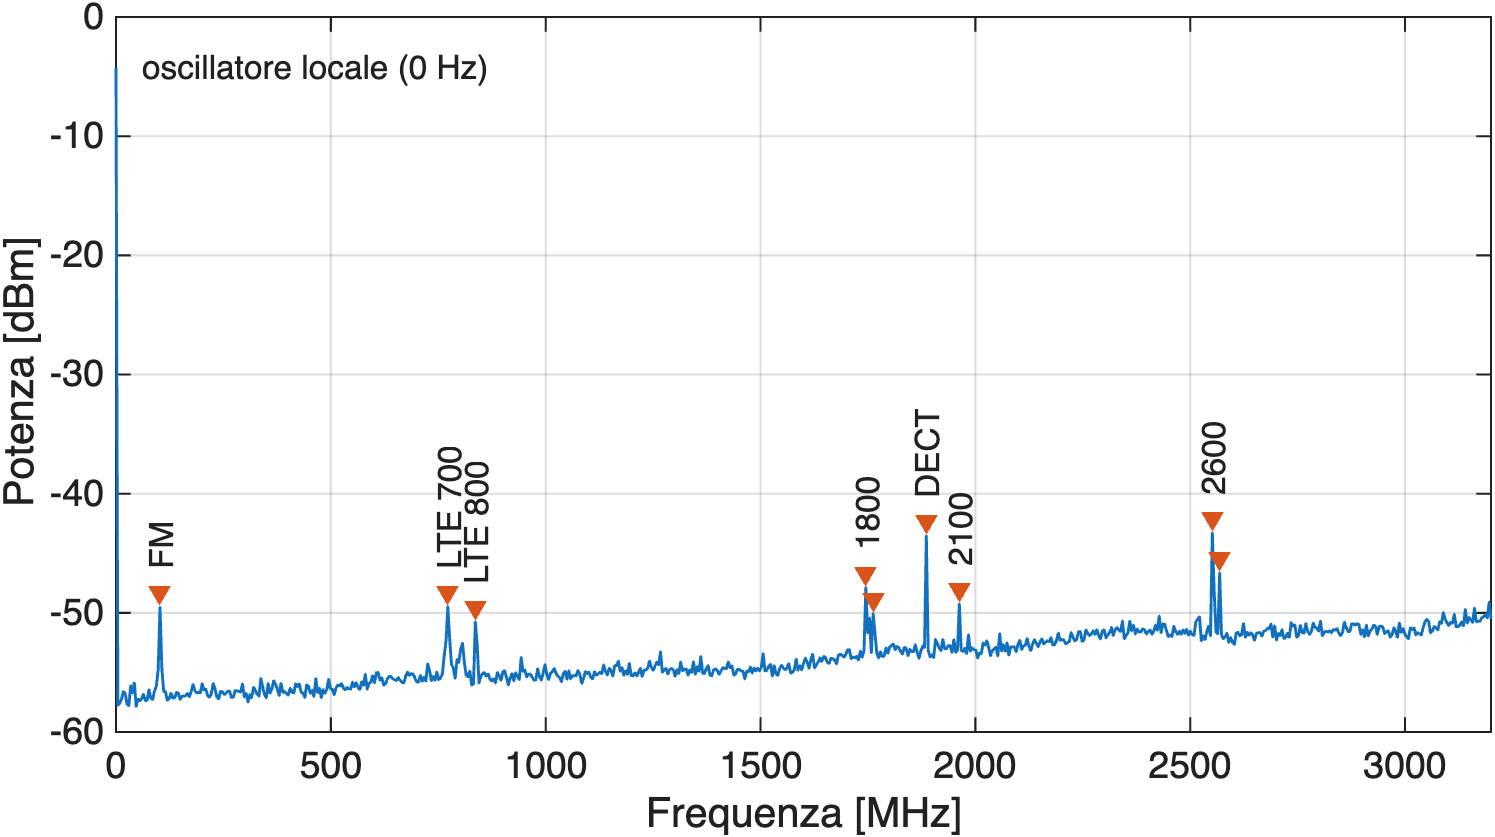
\includegraphics[width=\textwidth]{Images/Relazione2_Foto/5_1_full_span.png}
\caption{Punto 5.1: spettro ricevuto dall'antenna su tutta la banda dello SPA, traccia in max hold (751 punti, 4.27\,MHz fra due punti). I triangoli segnano i picchi almeno 3\,dB sopra il fondo; 1800, 2100 e 2600 sono le bande in cui trasmettono i telefoni cellulari.}
\label{fig:5_1_fullspan}
\end{figure}

\begin{table}[H]
\centering\small
\renewcommand{\arraystretch}{1.15}
\begin{tabular}{r r r l}
\hline
$f$ [MHz] & $P$ [dBm] & sopra il fondo [dB] & servizio (banda) \\ \hline
102.4  & $-49.5$ & 7.2 & radio FM (87.5--108\,MHz) \\
772.3  & $-49.5$ & 5.8 & LTE 700, stazioni base (758--788\,MHz) \\
836.3  & $-50.8$ & 4.4 & LTE 800, telefoni (832--862\,MHz) \\
1745.1 & $-47.9$ & 5.6 & GSM/LTE 1800, telefoni (1710--1785\,MHz) \\
1762.1 & $-50.1$ & 3.3 & GSM/LTE 1800, telefoni \\
1885.9 & $-43.5$ & 9.5 & DECT, telefoni cordless (1880--1900\,MHz) \\
1962.7 & $-49.2$ & 3.8 & UMTS/LTE 2100, telefoni (1920--1980\,MHz) \\
2551.5 & $-43.3$ & 8.5 & LTE 2600, telefoni (2500--2570\,MHz) \\
2568.5 & $-46.6$ & 5.1 & LTE 2600, telefoni \\ \hline
\end{tabular}
\caption{Picchi riconosciuti nella traccia di Fig.~\ref{fig:5_1_fullspan}. Incertezza sulla frequenza: $\pm 64$\,MHz con la formula della practice, $\pm 2.2$\,MHz con quella del datasheet dello SPA (vedi testo).}
\label{tab:5_1_picchi}
\end{table}

\paragraph{Incertezza.} La formula della practice, $\delta f = \pm(f\cdot 10^{-6} + 2\%\cdot\mathrm{SPAN} + 20\%\cdot\mathrm{RBW})$, in full span dà $\pm 64$\,MHz, quasi tutti dovuti al termine $2\%\cdot\mathrm{SPAN}$. Il datasheet dello SPA indica per la lettura della frequenza $\pm(f\cdot\delta_{\mathrm{ref}} + 10\%\cdot\mathrm{RBW} + \tfrac12\,\mathrm{SPAN}/750 + 1\,\mathrm{Hz}) \simeq \pm 2.2$\,MHz, dominato dalla distanza fra i punti. Il valore realistico è il secondo: il picco DECT, che qui cade a 1885.9\,MHz, con lo span di 10\,MHz del punto 5.4 si trova a 1883.5\,MHz, cioè 2.4\,MHz più in basso, circa mezzo passo della traccia. Le potenze sono solo indicative: i picchi superano il fondo di 3--10\,dB, mentre l'incertezza di $\pm 0.5$\,dB della practice vale per un rapporto segnale/rumore maggiore di 16\,dB.

\paragraph{Commento.} I segnali trovati sono quelli attesi. Le righe più alte sono quelle dei telefoni (bande di uplink a 1.8, 2.0 e 2.6\,GHz) e del DECT, sorgenti vicine e dentro l'edificio; delle stazioni base emerge solo quella LTE a 772\,MHz. La radio FM appare come un'unica riga a 102.4\,MHz perché a questa risoluzione tutta la banda cade in pochi punti: la risolviamo nel punto 5.2. Il Wi-Fi a 2.4\,GHz, che durante la misura abbiamo visto comparire sullo schermo, nella traccia salvata supera il fondo di soli 1.3\,dB; televisione, DAB+ e le altre bande delle stazioni base restano sotto il fondo, che in full span è alto perché la RBW è larga e il max hold conserva anche i massimi del rumore. Per vederli servirebbero uno span più stretto e una RBW più piccola, come nel punto successivo. La riga a 0\,Hz ($-4.3$\,dBm) non è un segnale ricevuto: è l'oscillatore locale dello SPA che passa attraverso il mixer fino al rivelatore.

% ---------------------------------------------------------------------
\section{Le tre radio FM più potenti (punto 5.2)}
\label{sec:5_2}

\paragraph{Che cosa ci aspettiamo.} A Roma la banda FM (87.5--108\,MHz) è quasi tutta occupata, con canali a passi di 100\,kHz; le emittenti più forti trasmettono da Monte Cavo, sui Castelli Romani, e da Monte Mario. Un'emittente FM occupa circa 200\,kHz: due massimi più vicini di 200\,kHz appartengono quindi allo stesso segnale.

\paragraph{Come abbiamo misurato.} Start 80\,MHz, stop 110\,MHz, traccia in max hold. Per separare le emittenti e abbassare il fondo abbiamo ridotto la RBW a 1\,kHz e portato l'attenuatore d'ingresso a 0\,dB: fuori dalla banda FM il fondo scende a circa $-102$\,dBm. Con 751 punti su 30\,MHz due punti distano 40\,kHz. Sulla traccia salvata lo script cerca i massimi locali, li ordina dal più alto e scarta quelli a meno di 200\,kHz da un massimo già scelto; la frequenza di ogni emittente è stimata come baricentro, pesato in potenza, dei punti entro 10\,dB dal massimo.

\begin{figure}[H]
\centering
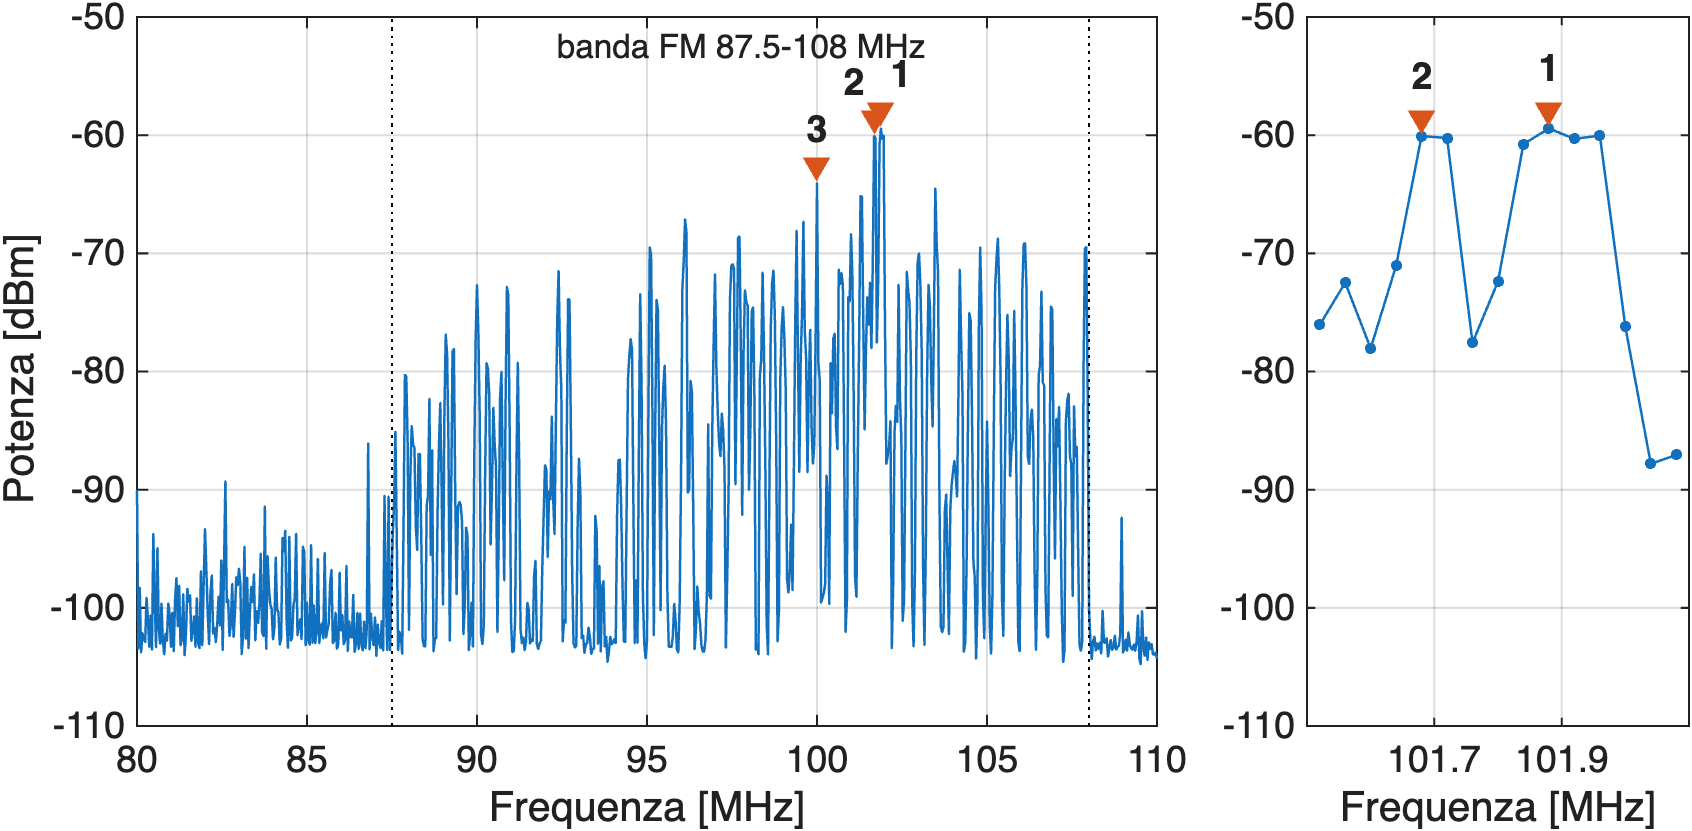
\includegraphics[width=\textwidth]{Images/Relazione2_Foto/5_2_banda_FM.png}
\caption{Punto 5.2: banda 80--110\,MHz in max hold, RBW 1\,kHz, attenuazione 0\,dB, 751 punti (40\,kHz fra due punti). A sinistra le tre emittenti più potenti trovate in MATLAB; a destra l'ingrandimento sulle emittenti 1 e 2, distanti 200\,kHz (i punti sono i campioni della traccia).}
\label{fig:5_2_fm}
\end{figure}

\begin{table}[H]
\centering\small
\renewcommand{\arraystretch}{1.15}
\begin{tabular}{c c c c l}
\hline
 & $f$ del massimo & $f$ baricentro & $P$ & emittente \\
 & [MHz] & [MHz] & [dBm] & (frequenza nominale) \\ \hline
1 & 101.88 & 101.901 & $-59.4 \pm 0.5$ & Dimensione Suono Roma (101.9\,MHz) \\
2 & 101.68 & 101.700 & $-60.1 \pm 0.5$ & Radio Evangelo Roma (101.7\,MHz) \\
3 & 100.00 & 100.000 & $-64.1 \pm 0.5$ & R101 (100.0\,MHz) \\ \hline
(4) & 103.48 & 103.499 & $-64.5 \pm 0.5$ & Rai Isoradio (103.5\,MHz) \\ \hline
\end{tabular}
\caption{Le tre emittenti FM più potenti; la quarta è riportata perché è a soli 0.4\,dB dalla terza. Tutte e quattro trasmettono da Monte Cavo.}
\label{tab:5_2_radio}
\end{table}


\paragraph{Verifica.} Le frequenze trovate coincidono con quelle nominali di tre emittenti romane, entro 20\,kHz per il massimo della traccia ed entro 1\,kHz per il baricentro; coincidono anche la quarta, la quinta e la sesta emittente in ordine di potenza (103.5, 101.3 e 96.1\,MHz). Questo confronto mostra che la scala delle frequenze dello SPA è precisa quanto dice il datasheet ($\pm 20$\,kHz, cioè mezzo passo della traccia).


% ---------------------------------------------------------------------
\setcounter{section}{3}% nella practice non c'è un punto 5.3
\section{Campo elettrico e magnetico (punto 5.4)}
\label{sec:5_4}

\subsection{Dalla potenza ricevuta al campo}
Il fattore d'antenna $AF$ lega il campo elettrico incidente alla tensione ai capi dello SPA, $E = AF \cdot V$; sui 50\,$\Omega$ d'ingresso $V^2 = 50\,P$. Esprimendo $P$ in dBm, $V$ in dB$\mu$V ($V = P + 107$) e $E$ in dBV/m (si sottraggono 120\,dB) si ottiene la formula della practice:
\begin{equation}
E\,[\mathrm{dBV/m}] = P_{RIC}\,[\mathrm{dBm}] + AF\,[\mathrm{dB/m}] - 13,
\qquad E\,[\mathrm{V/m}] = 10^{E[\mathrm{dBV/m}]/20}.
\label{eq:5_campo}
\end{equation}
Il fattore d'antenna del datasheet comprende già l'attenuazione del cavo. In campo lontano il campo magnetico è $H = E/\eta_0$, con $\eta_0 = 120\pi \simeq 377\,\Omega$.

L'antenna misura solo la componente del campo parallela al proprio asse. Il supporto ha tre posizioni a scatto, ruotate di $120^\circ$ attorno alla verticale, con l'asse dell'antenna inclinato di $\theta = 54.7^\circ$ sulla verticale (Fig.~\ref{fig:5_4_posizioni}): con questa inclinazione i tre assi sono a due a due ortogonali, come i tre spigoli di un cubo che escono dallo stesso vertice ($\cos^2\theta + \sin^2\theta\cos 120^\circ = \tfrac13 - \tfrac23\cdot\tfrac12 = 0$). Il modulo del campo si ottiene combinando in V/m le tre componenti:
\begin{equation}
|E| = \sqrt{E_1^2 + E_2^2 + E_3^2}, \qquad |H| = |E|/\eta_0 .
\label{eq:5_modulo}
\end{equation}

\begin{figure}[H]
\centering
\begin{tikzpicture}[>={Stealth[length=5pt]}]
  \begin{scope}
    \draw[->] (0,0) -- (0,2.5) node[above,font=\small] {verticale};
    \draw[->] (0,0) -- (2.5,0) node[right,font=\small] {orizzontale};
    \draw[very thick,blue!70!black] (215.26:1.3) -- (35.26:2.2) node[above right,font=\small] {asse dell'antenna};
    \draw (0,1.1) arc[start angle=90,end angle=35.26,radius=1.1];
    \node[font=\small] at (0.36,1.36) {$\theta$};
    \node[font=\small] at (1.2,-1.1) {$\cos\theta = 1/\sqrt3$, $\theta \simeq 54.7^\circ$};
    \node[font=\small] at (1.0,-2.3) {vista di lato};
  \end{scope}
  \begin{scope}[shift={(8,0.3)}]
    \draw[gray] (0,0) circle[radius=1.4];
    \foreach \a/\n in {0/0,120/120,240/240}{
      \draw[->,very thick,blue!70!black] (0,0) -- (\a:1.4);
      \node[font=\small] at (\a:2.15) {$\varphi=\n^\circ$};
    }
    \fill (0,0) circle[radius=1.5pt];
    \node[font=\small] at (0,-2.6) {vista dall'alto};
  \end{scope}
\end{tikzpicture}
\caption{Le tre posizioni dell'antenna: asse inclinato di $54.7^\circ$ sulla verticale e ruotato di $120^\circ$ da una posizione all'altra; i tre assi sono a due a due ortogonali.}
\label{fig:5_4_posizioni}
\end{figure}

\subsection{Scelta del segnale e impostazioni}
\paragraph{Il segnale.} Nella traccia full span acquisita con l'antenna nella prima posizione la riga più alta, esclusa quella a 0\,Hz, è a 1881.6\,MHz ($-45.3$\,dBm): è il DECT già visto nel punto 5.1, un segnale vicino e stabile, e lo abbiamo scelto per la misura del campo.

\paragraph{Che cosa ci aspettiamo.} Un apparecchio DECT trasmette al massimo 250\,mW di picco (24\,dBm). In spazio libero, a distanza $d$, una sorgente con potenza irradiata $P_{EIRP}$ produce $E = \sqrt{30\,P_{EIRP}}/d \simeq 2.7\,\mathrm{V}/d[\mathrm{m}]$: per una sorgente a 5--25\,m ci aspettiamo $|E|$ fra circa 0.1 e 0.5\,V/m. A 1.88\,GHz la lunghezza d'onda è 16\,cm, quindi a queste distanze siamo in campo lontano e la relazione $H = E/\eta_0$ vale.

\paragraph{Come abbiamo misurato.} Centro 1.88\,GHz, span 10\,MHz (con uno span di 2\,MHz il canale non entrava tutto nello schermo; con 10\,MHz si vede anche il fondo ai lati), RBW 300\,kHz come chiede la practice, attenuazione 0\,dB e traccia in max hold. Per ognuna delle tre posizioni abbiamo azzerato il max hold e salvato la traccia (Fig.~\ref{fig:5_4_tracce}); che l'azzeramento sia avvenuto lo conferma la traccia a $120^\circ$, più bassa di quella a $0^\circ$ in quasi tutto il canale. I massimi cadono fra 1883.47 e 1883.55\,MHz, a meno di 60\,kHz dalla portante DECT a 1883.520\,MHz (le portanti europee sono $1897.344 - c\cdot 1.728$\,MHz, qui $c = 8$): con un segnale modulato largo circa 1\,MHz il massimo della traccia non coincide esattamente con la portante.

\begin{figure}[H]
\centering
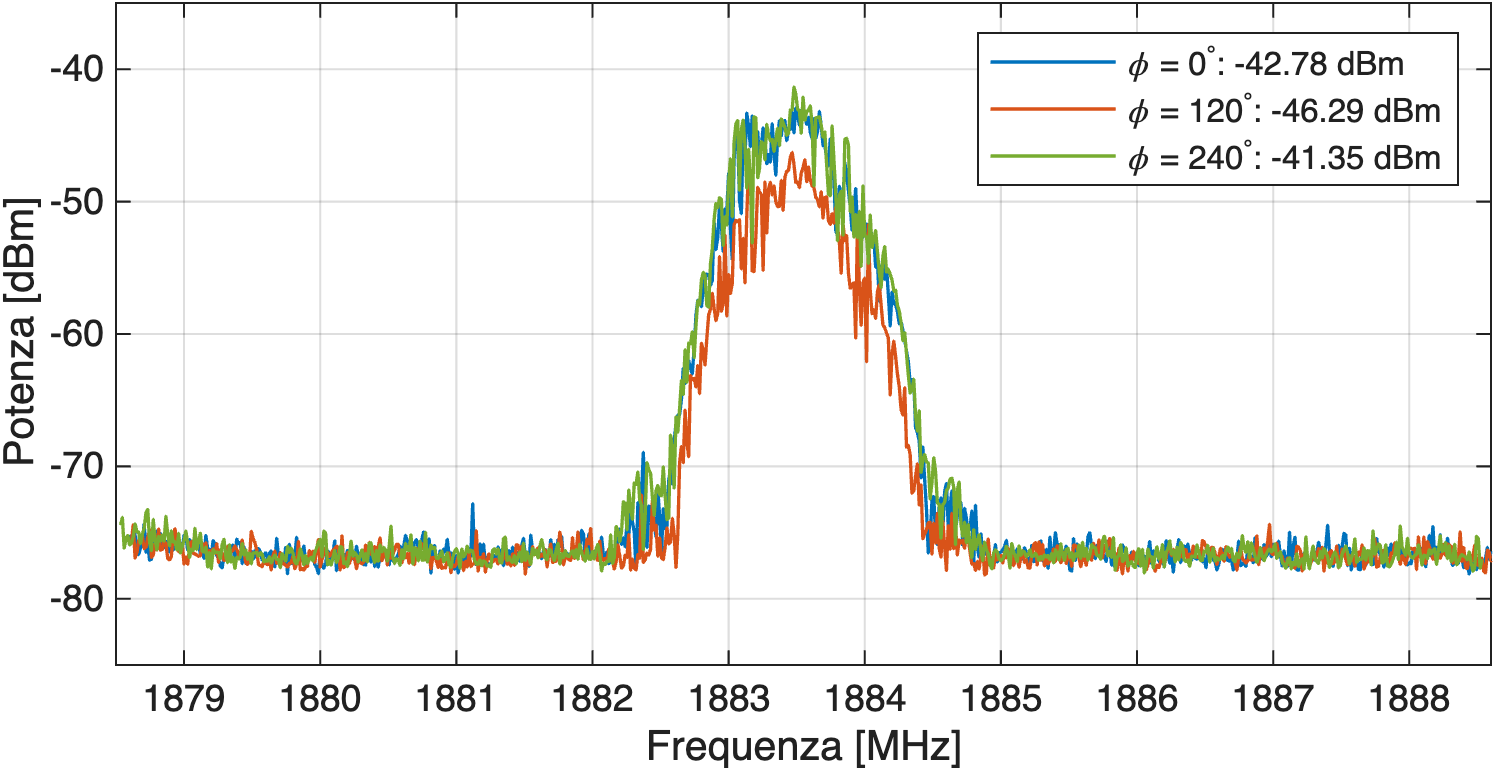
\includegraphics[width=\textwidth]{Images/Relazione2_Foto/5_4_tre_posizioni.png}
\caption{Punto 5.4: il segnale DECT nelle tre posizioni dell'antenna; span 10\,MHz, RBW 300\,kHz, attenuazione 0\,dB, max hold, 751 punti. In legenda il massimo di ciascuna traccia.}
\label{fig:5_4_tracce}
\end{figure}

\subsection{Risultati}
Il fattore d'antenna a 1883.5\,MHz, interpolato sulla curva del datasheet (Fig.~\ref{fig:5_4_af}), è $AF = 39.0$\,dB/m. Con la (\ref{eq:5_campo}) si ottengono i valori della Tabella~\ref{tab:5_4_campo}.

\begin{figure}[H]
\centering
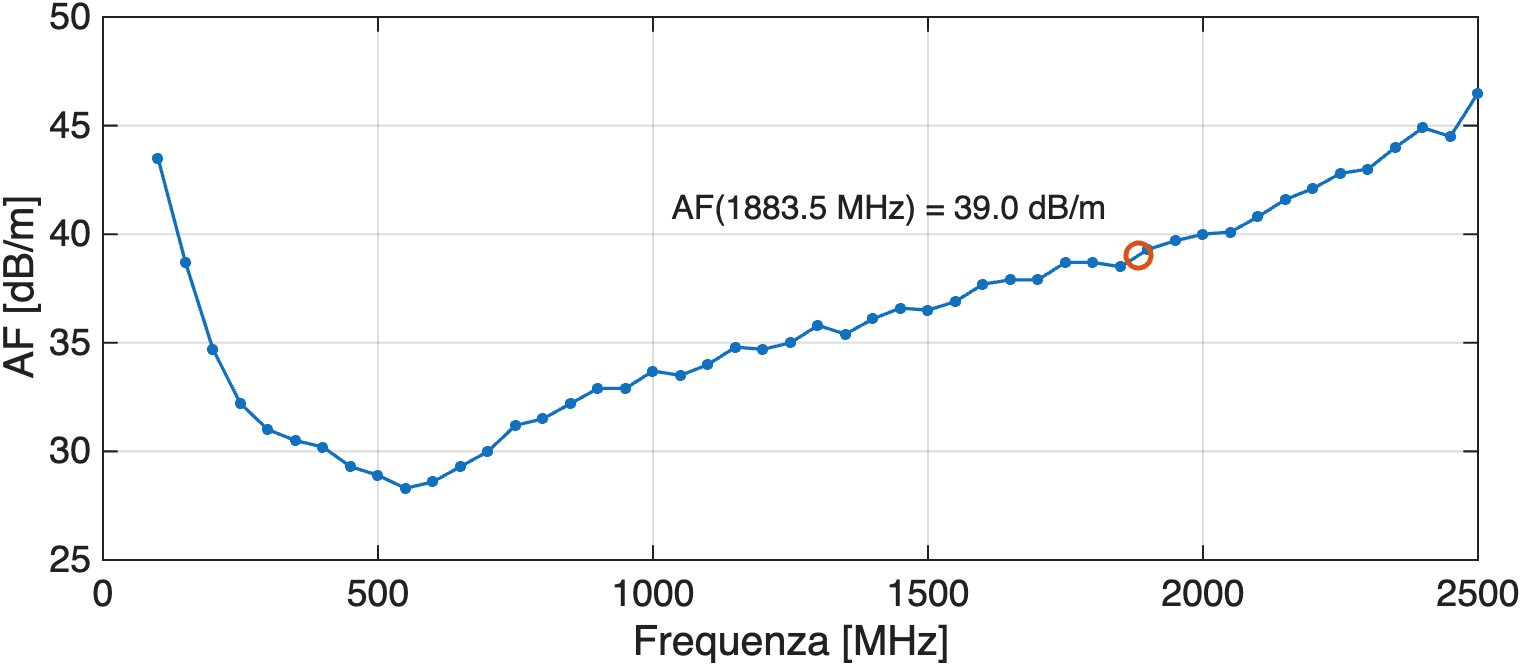
\includegraphics[width=0.85\textwidth]{Images/Relazione2_Foto/5_4_fattore_antenna.png}
\caption{Fattore d'antenna (cavo compreso) letto sul grafico del datasheet allegato alla practice, a passi di 50\,MHz, e valore interpolato alla frequenza del segnale.}
\label{fig:5_4_af}
\end{figure}

\begin{table}[H]
\centering
\renewcommand{\arraystretch}{1.2}
\begin{tabular}{c c c c c c}
\hline
posizione & $f$ [MHz] & $P_{RIC}$ [dBm] & $E$ [dBV/m] & $E$ [mV/m] & $H$ [mA/m] \\ \hline
$\varphi = 0^\circ$   & 1883.55 & $-42.78$ & $-16.8^{+2.4}_{-3.3}$ & $145 \pm 46$ & $0.38 \pm 0.12$ \\
$\varphi = 120^\circ$ & 1883.47 & $-46.29$ & $-20.3^{+2.4}_{-3.3}$ & $97 \pm 31$  & $0.256 \pm 0.082$ \\
$\varphi = 240^\circ$ & 1883.48 & $-41.35$ & $-15.4^{+2.4}_{-3.3}$ & $171 \pm 54$ & $0.45 \pm 0.14$ \\ \hline
modulo & & & $-12.3^{+1.6}_{-1.9}$ & $244 \pm 48$ & $0.65 \pm 0.13$ \\ \hline
\end{tabular}
\caption{Potenza ricevuta e campo nelle tre posizioni dell'antenna, con $AF = 39.0$\,dB/m; il modulo è calcolato in V/m con la (\ref{eq:5_modulo}). Incertezze estese con $k = 2$ (\S\ref{sec:5_4_incertezza}); in dB l'intervallo è asimmetrico: $\pm 32\,\%$ sul campo corrisponde a $+2.4/-3.3$\,dB.}
\label{tab:5_4_campo}
\end{table}

\subsection{Incertezza}
\label{sec:5_4_incertezza}
Ogni componente è una misura diretta. La practice dà tre contributi, che convertiamo in incertezza relativa sul campo (una grandezza di tensione, quindi $\pm a$\,dB corrisponde a $10^{a/20} - 1$) e dividiamo per il fattore della rispettiva distribuzione, (come nelle slide del corso) (Tabella~\ref{tab:5_4_budget}).

\begin{table}[H]
\centering
\renewcommand{\arraystretch}{1.2}
\begin{tabular}{l c c c c c}
\hline
contributo & $\pm a$ & distribuzione & $10^{a/20}-1$ & divisore & $u_i$ \\ \hline
fattore d'antenna & 2\,dB & normale & 25.9\,\% & 2 & 12.9\,\% \\
AF interpolato & 0.5\,dB & rettangolare & 5.9\,\% & $\sqrt3$ & 3.4\,\% \\
disadattamento & 1\,dB & a U & 12.2\,\% & $\sqrt2$ & 8.6\,\% \\ \hline
\multicolumn{5}{l}{incertezza tipo relativa di ogni componente, $u_r = \sqrt{\textstyle\sum u_i^2}$} & 15.9\,\% \\ \hline
\end{tabular}
\caption{Bilancio d'incertezza di una componente del campo.}
\label{tab:5_4_budget}
\end{table}

Con $k = 2$ l'incertezza estesa di ogni componente è $31.9\,\%$, cioè $+2.4/-3.3$\,dB. Il modulo è una misura indiretta: propagando l'incertezza nella (\ref{eq:5_modulo}) con le tre componenti indipendenti, come nelle slide del corso,
\begin{equation}
u_r(|E|) = \frac{\sqrt{E_1^4 u_{r}^2 + E_2^4 u_{r}^2 + E_3^4 u_{r}^2}}{|E|^2}
         = u_r\,\frac{\sqrt{E_1^4 + E_2^4 + E_3^4}}{|E|^2} = 15.9\,\% \times 0.624 = 9.9\,\%,
\end{equation}
e con $k = 2$ l'incertezza estesa è $U = 19.9\,\%$:
\begin{equation}
|E| = (0.244 \pm 0.048)\ \mathrm{V/m}, \qquad |H| = (0.65 \pm 0.13)\ \mathrm{mA/m} \qquad (k = 2).
\end{equation}

\subsection{Commento}
Il risultato rientra nell'intervallo atteso: con 250\,mW di picco, $|E| = 0.244$\,V/m corrisponde a una sorgente a circa 11\,m, compatibile con un apparecchio DECT nell'edificio. Le tre componenti hanno pesi diversi (il 49\,\% della potenza cade sulla posizione a $240^\circ$, il 16\,\% su quella a $120^\circ$): il campo è polarizzato, come ci si aspetta da un singolo trasmettitore.

% =====================================================================
%  CAPITOLO 6 - Armoniche di un diodo Schottky
%  Script e dati: MatLab/2_Exp (punto6_armoniche_diodo.m)
%  Figura: Images/Relazione2_Foto/6_armoniche_diodo.png
% =====================================================================
\chapter{Risposta in frequenza di un diodo Schottky}
\chaptermark{Armoniche di un diodo Schottky}
\label{cap:diodo}

Un diodo è un componente non lineare: se lo si eccita con una sinusoide a frequenza $f_0$, la corrente che lo attraversa contiene anche componenti a $2f_0$, $3f_0$ e così via. In questa misura abbiamo eccitato un diodo Schottky con un tono a $f_0 = 800$\,MHz e abbiamo misurato con lo SPA la potenza della seconda e della terza armonica rispetto a quella della fondamentale.

\section{Che cosa ci aspettiamo}
La caratteristica del diodo è esponenziale, $i = I_s\left(e^{v/(nV_T)} - 1\right)$. Per tensioni piccole rispetto a $nV_T$ la si può sviluppare in serie,
\begin{equation}
i(v) \simeq a_1 v + a_2 v^2 + a_3 v^3 + \dots, \qquad a_k = \frac{I_s}{k!\,(nV_T)^k},
\end{equation}
e con $v = V\cos\omega_0 t$ i termini di grado superiore producono nuove frequenze:
\begin{equation}
v^2 = \frac{V^2}{2}\left(1 + \cos 2\omega_0 t\right), \qquad
v^3 = \frac{V^3}{4}\left(3\cos\omega_0 t + \cos 3\omega_0 t\right).
\end{equation}
La seconda armonica nasce dal termine quadratico ed è proporzionale a $V^2$, la terza dal termine cubico ed è proporzionale a $V^3$. Ci aspettiamo quindi righe a $2f_0$ e $3f_0$ via via più basse; in potenza, finché lo sviluppo vale, la seconda armonica cresce di 2\,dB e la terza di 3\,dB per ogni dB di potenza incidente, quindi i livelli in dBc dipendono dalla potenza con cui si pilota il diodo.

\section{Set-up}
Lo schema è quello della practice (Fig.~\ref{fig:6_setup}). La sorgente, l'analizzatore di reti PNA del banco usato come generatore a frequenza fissa , è collegata alla porta OUT dell'accoppiatore direzionale, il diodo alla porta IN e lo SPA alla porta accoppiata CPL. L'accoppiatore è quindi montato al contrario rispetto al suo verso di misura:
\begin{itemize}
  \item l'onda della sorgente viaggia da OUT verso IN e raggiunge il diodo, ma verso CPL passa solo attraverso la direttività finita dell'accoppiatore, cioè molto attenuata: lo SPA non riceve la potenza piena della sorgente;
  \item ciò che torna dal diodo, la fondamentale riflessa e le armoniche generate, viaggia da IN verso OUT, cioè nel verso accoppiato, e arriva su CPL attenuato del solo fattore di accoppiamento.
\end{itemize}
Così lo SPA vede soprattutto il segnale prodotto dal diodo, e fondamentale e armoniche arrivano su CPL per lo stesso percorso: il loro rapporto in dBc è, a meno della risposta in frequenza dell'accoppiatore, quello presente alla porta del diodo.

\begin{figure}[H]
\centering
\begin{tikzpicture}[>={Stealth[length=5pt]},
  box/.style={draw,thick,rounded corners=2pt,minimum height=1.2cm,minimum width=2.5cm,align=center,font=\small}]
  \node[box] (src) at (0,0) {Sorgente\\$f_0 = 800$\,MHz};
  \node[box,minimum width=3.4cm,minimum height=1.5cm] (cpl) at (4.7,0) {};
  \node[font=\small,align=center] at (4.7,-0.2) {Accoppiatore\\direzionale};
  \node[font=\scriptsize,anchor=west] at ([yshift=0.3cm]cpl.west) {OUT};
  \node[font=\scriptsize,anchor=east] at ([yshift=0.3cm]cpl.east) {IN};
  \node[font=\scriptsize,anchor=north] at (cpl.north) {CPL};
  \node[box] (d) at (9.4,0) {Diodo\\Schottky};
  \node[box] (sa) at (4.7,2.7) {SPA};
  \draw[thick] (src.east) -- (cpl.west);
  \draw[thick] (cpl.east) -- (d.west);
  \draw[thick] (cpl.north) -- (sa.south);
  \draw[->,red!70!black,thick] (6.7,-1.1) -- node[below,font=\scriptsize,align=center]{onda incidente a $f_0$\\(OUT$\to$IN, isolata da CPL)} (8.3,-1.1);
  \draw[->,blue!70!black,thick] (8.3,1.1) -- node[above,font=\scriptsize,align=center]{$f_0$ riflessa, $2f_0$, $3f_0$\\(IN$\to$OUT, accoppiate su CPL)} (6.7,1.1);
\end{tikzpicture}
\caption{Set-up della misura 6, con l'accoppiatore montato al contrario.}
\label{fig:6_setup}
\end{figure}

\section{Scelta della frequenza e impostazioni}
Le prime tre armoniche devono cadere nella banda dell'accoppiatore, che parte da circa 0.7\,GHz, e la terza anche sotto il limite dello SPA, 3.2\,GHz. Quindi $f_0 \gtrsim 0.7$\,GHz e $3f_0 \le 3.2$\,GHz, cioè $f_0 \lesssim 1.07$\,GHz: abbiamo scelto $f_0 = 800$\,MHz, con le righe a 0.8, 1.6 e 2.4\,GHz.

Sullo SPA abbiamo impostato start 400\,MHz e stop 2.8\,GHz (da $f_0/2$ a $3.5\,f_0$), RBW 30\,kHz per tenere basso il fondo (circa $-86$\,dBm) e attenuazione 0\,dB. Con 751 punti su 2.4\,GHz due punti distano 3.2\,MHz, e con questo span le tre frequenze cadono esattamente su punti della traccia ($400 + 3.2\,n$\,MHz). La RBW stretta rende la scansione lenta, qualche secondo, ma con un tono fisso non è un problema.

\section{Risultati}
I livelli delle tre righe sono nella Tabella~\ref{tab:6_armoniche}; la traccia acquisita è in Fig.~\ref{fig:6_armoniche}.

\begin{table}[H]
\centering
\renewcommand{\arraystretch}{1.2}
\begin{tabular}{c c c c c}
\hline
riga & $f$ [MHz] & $P$ [dBm] & rispetto a $f_0$ [dBc] & segnale/rumore [dB] \\ \hline
$f_0$  & 800  & $-47.8 \pm 0.5$ & 0 & 39 \\
$2f_0$ & 1600 & $-69.3 \pm 0.5$ & $-21.5 \pm 0.8$ & 17 \\
$3f_0$ & 2400 & $-75.7$ & $-27.9$ & 7 \\ \hline
\end{tabular}
\caption{Livelli delle prime tre armoniche alla porta CPL. Incertezze estese ($k = 2$); per la terza armonica vedi il testo.}
\label{tab:6_armoniche}
\end{table}

\begin{figure}[H]
\centering
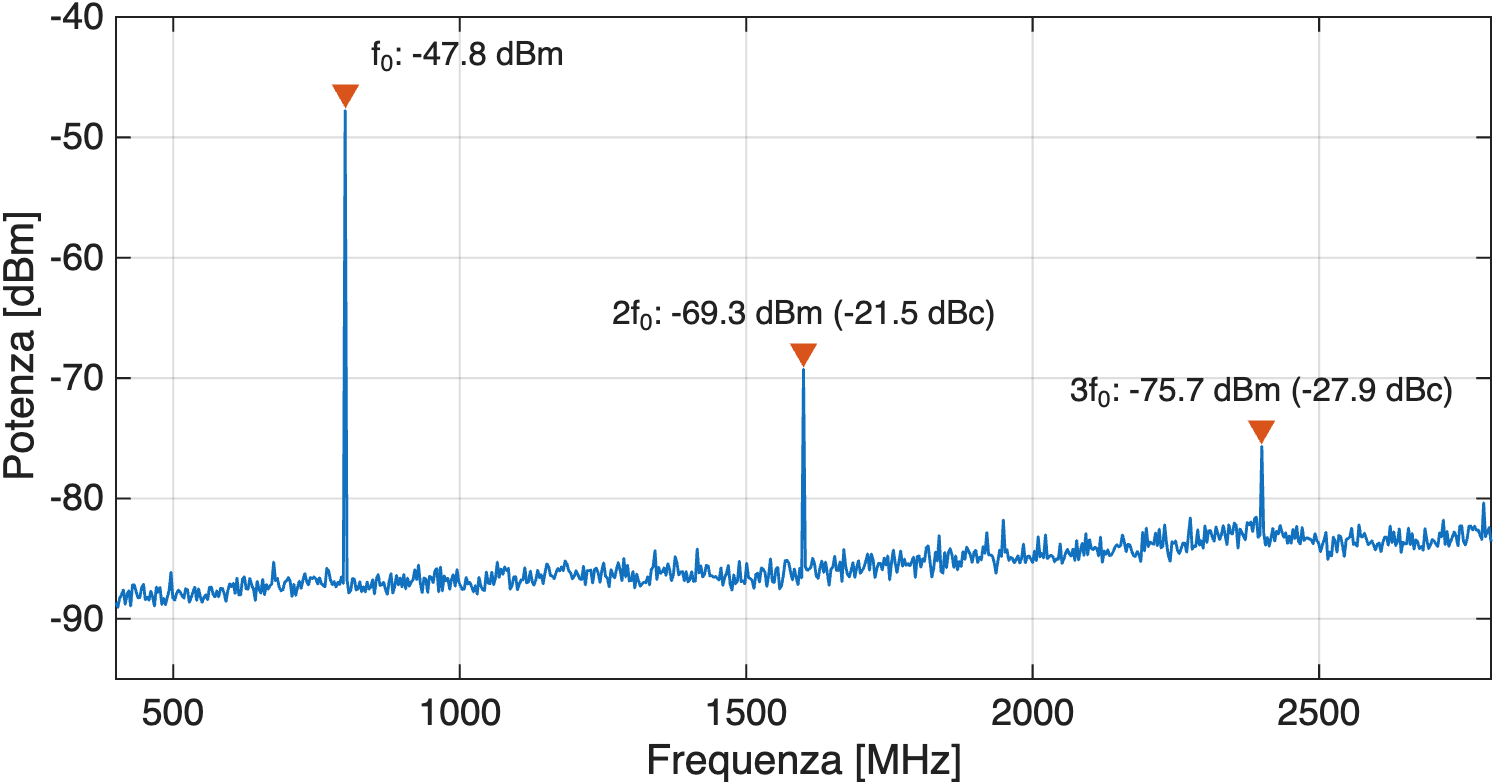
\includegraphics[width=\textwidth]{Images/Relazione2_Foto/6_armoniche_diodo.png}
\caption{Punto 6: spettro alla porta CPL con il diodo pilotato a $f_0 = 800$\,MHz; start 400\,MHz, stop 2.8\,GHz, RBW 30\,kHz, attenuazione 0\,dB, 751 punti.}
\label{fig:6_armoniche}
\end{figure}

\paragraph{Incertezza.} Per ogni livello la practice indica un errore massimo di $\pm 0.5$\,dB, valido se il rapporto segnale/rumore supera 16\,dB. Il rapporto in dBc è la differenza di due letture: con distribuzione rettangolare $u = \sqrt2 \cdot 0.5/\sqrt3 = 0.41$\,dB, e con $k = 2$ l'incertezza estesa è $\pm 0.8$\,dB. La terza armonica supera il fondo di soli 7\,dB, fuori dalle condizioni della practice: il rumore che si somma alla riga ne alza la lettura di circa 0.9\,dB, e togliendo il contributo del fondo il livello diventa $-76.6$\,dBm, cioè $-28.8$\,dBc.

\paragraph{Da dove vengono le armoniche.} Per attribuire le righe al diodo bisogna escludere le altre due sorgenti possibili.
\begin{itemize}
  \item \textbf{Lo SPA.} Il suo mixer genera armoniche se il segnale d'ingresso è forte. Qui la fondamentale arriva a $-47.8$\,dBm con attenuazione 0\,dB: con un intercetto di seconda armonica di $+45$\,dBm (datasheet), la seconda armonica prodotta dallo strumento sarebbe $2 \times (-47.8) - 45 \simeq -141$\,dBm, ben sotto il fondo.
  \item \textbf{La sorgente.} Anche il generatore produce armoniche, che seguono lo stesso percorso della fondamentale. Nella traccia \texttt{Prima\_Misura}, la prova di acquisizione fatta all'inizio dell'esercitazione con la sorgente del banco a 800\,MHz collegata allo SPA (fondamentale a $-1.2$\,dBm), le armoniche della sorgente sono a $-41.0$\,dBc (seconda) e $-37.8$\,dBc (terza): 19.5\,dB e 9.9\,dB sotto quelle misurate con il diodo. Se nel punto 6 la sorgente lavorava alla stessa potenza, queste righe, sommandosi in ampiezza con fase ignota a quelle del diodo, possono spostare la seconda armonica di circa $\pm 1$\,dB e la terza fino a $+2.4/-3.4$\,dB.
\end{itemize}
La seconda armonica è quindi una misura solida del diodo: $(-21.5 \pm 0.8)$\,dBc, con al più 1\,dB di incertezza aggiuntiva dovuta alla sorgente. La terza è indicativa: fra $-28$ e $-29$\,dBc con un'incertezza di qualche dB.

\section{Commento}
I risultati sono quelli attesi: le armoniche ci sono e decrescono con l'ordine, la terza più bassa della seconda. Il confronto in dBc risente della risposta in frequenza dell'accoppiatore, dei cavi e dello SPA fra 0.8 e 2.4\,GHz, che non abbiamo calibrato (per lo SPA il datasheet indica una planarità di $\pm 0.8$\,dB). Inoltre i valori in dBc valgono per la potenza di sorgente usata: poiché la seconda armonica cresce di 2\,dB e la terza di 3\,dB per ogni dB in più, ripetere la misura a due o tre potenze diverse permetterebbe di verificare queste pendenze. Infine, una misura con un carico da 50\,$\Omega$ al posto del diodo avrebbe dato direttamente il residuo dovuto a sorgente e accoppiatore, da sottrarre alle righe misurate.


\end{document}

